\chapter{The title of chapter two}

Lorem ipsum dolor sit amet, consectetuer adipiscing elit. Morbi commodo, ipsum sed pharetra gravida, orci magna rhoncus neque, id pulvinar odio lorem non turpis. Nullam sit amet enim. Suspendisse id velit vitae ligula volutpat condimentum. Aliquam erat volutpat. Sed quis velit. Nulla facilisi. Nulla libero. Vivamus pharetra posuere sapien \cite{hartley2003multiple}. Nam consectetuer. Sed aliquam, nunc eget euismod ullamcorper, lectus nunc ullamcorper orci, fermentum bibendum enim nibh eget ipsum. Donec porttitor ligula eu dolor. Maecenas vitae nulla consequat libero cursus venenatis. Nam magna enim, accumsan eu, blandit sed, blandit a, eros.

\section{Section 1}
Pellentesque habitant morbi tristique senectus et netus et malesuada fames ac turpis egestas. Vestibulum tortor quam, feugiat vitae, ultricies eget, tempor sit amet, ante. Donec eu libero sit amet quam egestas semper. Aenean ultricies mi vitae est. Mauris placerat eleifend leo. Quisque sit amet est et sapien ullamcorper pharetra. Vestibulum erat wisi, condimentum sed, commodo vitae, ornare sit amet, wisi \ref{fig:monitoringfrequencies}. Aenean fermentum, elit eget tincidunt condimentum, eros ipsum rutrum orci, sagittis tempus lacus enim ac dui. Donec non enim in turpis pulvinar facilisis. Ut felis.

\begin{figure}[H]
    \begin{subfigure}{.5\textwidth}
        \centering
        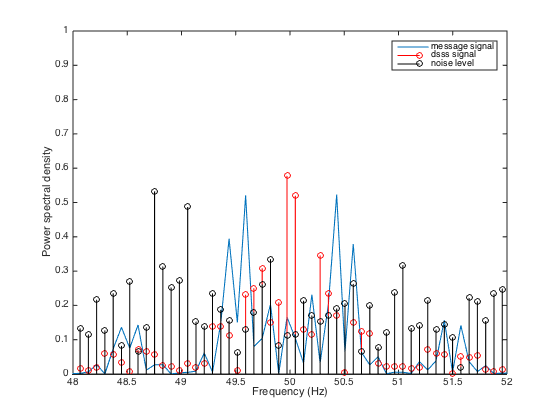
\includegraphics[width=1\linewidth]{images/figure1}
        \caption{Monitoring at 1khz.}
    \end{subfigure}
    \begin{subfigure}{.5\textwidth}
        \centering
        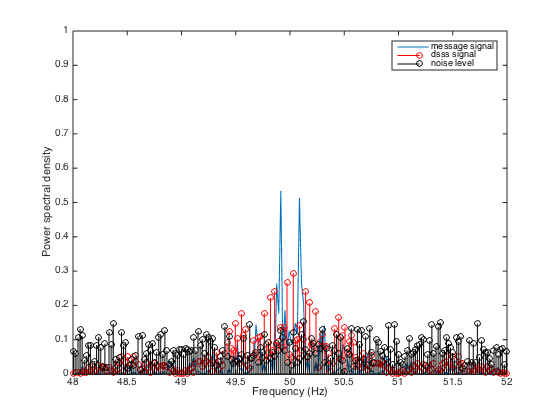
\includegraphics[width=1\linewidth]{images/figure2}
        \caption{Monitoring at 100khz.}
    \end{subfigure}
    \caption{Monitoring at different frequencies.}
    \label{fig:monitoringfrequencies}
\end{figure}

Cras sed ante. Phasellus in massa. Curabitur dolor eros, gravida et, hendrerit ac, cursus non, massa. Aliquam lorem. In hac habitasse platea dictumst. Cras eu mauris. Quisque lacus. Donec ipsum. Nullam vitae sem at nunc pharetra ultricies. Vivamus elit eros, ullamcorper a, adipiscing sit amet, porttitor ut, nibh. Maecenas adipiscing mollis massa. Nunc ut dui eget nulla venenatis aliquet. Sed luctus posuere justo. Cras vehicula varius turpis. Vivamus eros metus, tristique sit amet, molestie dignissim, malesuada et, urne \cite{hinton2006fast}

\section{Section 2}
Cras dictum. Maecenas ut turpis. In vitae erat ac orci dignissim eleifend. Nunc quis justo. Sed vel ipsum in purus tincidunt pharetra. Sed pulvinar, felis id consectetuer malesuada, enim nisl mattis elit, a facilisis tortor nibh quis leo. Sed augue lacus, pretium vitae, molestie eget, rhoncus quis, elit. Donec in augue. Fusce orci wisi, ornare id, mollis vel, lacinia vel, massa.

The selected points are then rearranged into a matrix:
\[
PH = \begin{bmatrix}
-x_1 & -y_1 & -1 & 0 & 0 & 0 & x_1 x_1' & y_1 x_1' & x_1' \\
0 & 0 & 0 & -x_1 & -y_1 & -1 & x_1 y_1' & y_1 y_1' & y_1' \\
-x_2 & -y_2 & -1 & 0 & 0 & 0 & x_2 x_2' & y_2 x_2' & x_2' \\
0 & 0 & 0 & -x_2 & -y_2 & -1 & x_2 y_2' & y_2 y_2' & y_2' \\
-x_3 & -y_3 & -1 & 0 & 0 & 0 & x_3 x_3' & y_3 x_3' & x_3' \\
0 & 0 & 0 & -x_3 & -y_3 & -1 & x_3 y_3' & y_3 y_3' & y_3' \\
-x_4 & -y_4 & -1 & 0 & 0 & 0 & x_4 x_4' & y_4 x_4' & x_4' \\
0 & 0 & 0 & -x_4 & -y_4 & -1 & x_4 y_4' & y_4 y_4' & y_4' 
\end{bmatrix}
\begin{bmatrix}
h1 \\ h2 \\ h3 \\ h4 \\ h5 \\ h6 \\ h7 \\ h8
\end{bmatrix} = 0
\]

Integer et accumsan ante. Integer sit amet tortor ex. Curabitur maximus pretium erat eget tristique. Aliquam erat volutpat. Sed tincidunt tempor tortor vel lobortis. Suspendisse potenti \ref{tab:truthtable}. Donec egestas, libero id gravida porta, erat quam laoreet diam, ac tincidunt velit lacus id mi. Praesent vulputate ante justo, ac blandit neque egestas sed. Pellentesque sed massa condimentum, consequat urna eget, venenatis nunc. Vivamus pharetra, tortor vitae sagittis bibendum, metus dui hendrerit arcu, vel gravida arcu ex ac enim. Fusce consectetur volutpat sagittis \cite{goldberg1988genetic}.

\begin{table}[ht]
    \centering
    \begin{tabular}{|l|l|l|l|l|} 
        \hline
        \multicolumn{2}{|c|}{input} & \multicolumn{2}{c|}{output} & \\
        \hline
        left & right & left & right & resulting movement\\ \hline
        0 & 0 & 1 & 1 & move forward\\ \hline
        0 & 1 & 1 & 0 & turn left\\ \hline
        1 & 0 & 0 & 1 & turn right\\ \hline
        1 & 1 & 0 & 0 & move backward\\ \hline
    \end{tabular}
    \caption{I/O truth table}
    \label{tab:truthtable}
\end{table}

Praesent ac risus venenatis, auctor diam eu, placerat purus. Pellentesque at elementum sem. Vivamus interdum augue augue, ut fringilla nisi tristique at. Maecenas ultricies rutrum purus, nec luctus diam. Nunc condimentum lobortis massa ut consequat. Curabitur quis tellus nibh. Vestibulum augue ante, vulputate ac felis faucibus, dapibus blandit magna. Pellentesque vitae augue fringilla, eleifend orci vitae, gravida arcu. Donec molestie nunc in orci sagittis ornare. Donec ultricies lorem interdum semper venenatis. Suspendisse sed neque gravida, ultrices purus vel, auctor nulla. Sed dapibus ornare interdum. Nullam eu ligula dapibus, semper libero vel, malesuada velit. Donec egestas augue libero, non commodo ante accumsan eu. Cras fringilla nisl non mollis elementum.

The metrics to collect are :
\begin{itemize}
    \item The gaze position of the subject
    \item The environment directly faced by each subject (RGB and depth)
    \item The position of each subject in the environment
\end{itemize}

Nullam sed egestas nunc. Ut vulputate laoreet leo, ut auctor nisi dictum non. Sed sit amet molestie elit. Pellentesque dictum magna nec nisl faucibus iaculis. Suspendisse lacinia convallis ipsum. Aenean vitae tristique risus. Duis tristique gravida euismod. Donec in purus pulvinar, blandit magna vel, congue nisi.